% 声明为子文件,指定主文件
\documentclass[main.tex]{subfiles}

% Ensure tikz/pgfplots are available so the "axis" environment is defined
\usepackage{tikz}
\usepackage{pgfplots}
\pgfplotsset{compat=1.18}

\begin{document}
\pagestyle{plain}
\setcounter{chapter}{3}

\chapter{Fixed point iteration. [2.2]}
\label{chap:lecture3}
\begin{definition}
    Let $D \subseteq \mathbb{R}$ and $f: D \rightarrow \mathbb{R}$ be a function. A point $p\in D$ is called a \textbf{fixed point} of $f$ if 
    \begin{equation}
        f(p) = p
    \end{equation}
\end{definition}

\begin{example}\par 
    \begin{enumerate}
        \item Any point $p\in \mathbb{R}$ is a fixed point of $f(x) = x$, the identity function. 
        \item Let $f(x) = x^2 - 2$. Then fixed points of $f$ satisfy 
        \begin{equation}
            p = f(p) = p^2 - 2 \Longleftrightarrow p^2 - p - 2 = (p + 1)(p - 2) = 0 \Longleftrightarrow p = -1 \text{ or } p = 2
        \end{equation}
        which can be graphically shown as follows:
        \begin{center}
            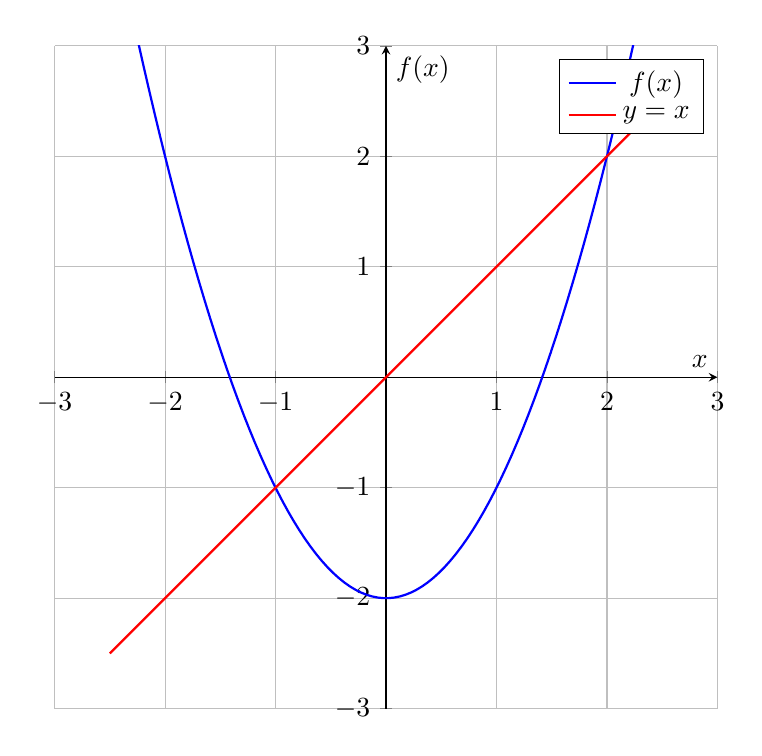
\begin{tikzpicture}
                \begin{axis}[
                    axis lines = middle,
                    xlabel = $x$,
                    ylabel = {$f(x)$},
                    ymin = -3, ymax = 3,
                    xmin = -3, xmax = 3,
                    domain = -2.5:2.5,
                    samples = 100,
                    grid = major,
                    width=10cm,
                    height=10cm,
                ]
                \addplot[domain=-2.5:2.5, samples=100, thick, blue] {x^2 - 2};
                \addplot[domain=-2.5:2.5, samples=100, thick, red] {x};
                \legend{$f(x)$, $y=x$}
                \end{axis}
            \end{tikzpicture}
        \end{center}
    \end{enumerate}
\end{example}

\begin{theorem}
    [Existence and Uniqueness]
    \begin{enumerate}
        \item If $f: [a, b] \rightarrow [a, b]$ is continuous, then $f$ has at least one fixed point in $[a, b]$.
        \item If $f'(x)$ exists on $(a, b)$ and there exists a constant $0 < k < 1$ such that $|f'(x)| \le k$ for all $x\in (a, b)$, then $f$ has one unique fixed point in $[a, b]$.
    \end{enumerate}
\end{theorem}
\par \noindent \textbf{Proof}
\par If $f(a) = a$ or $f(b) = b$, then we are done. 
\par We may assume that $f(a) > a$ and $f(b) < b$. Define $h(x) = f(x) - x$ which is continuous on $[a, b]$, with $h(a) = f(a) - a > 0$ and $h(b) = f(b) - b < 0$. By Bolzano's Intermediate Value Theorem, there exists $c\in (a, b)$ such that $h(c) = 0$, i.e. $f(c) = c$. This proves part 1.
\par Suppose that $|f'(x)|\le k < 1$, and that $p, q$ are both fixed points of $f$. We need to show that $p = q$. 
\par We assume the contrary that $p \neq q$. Without loss of generality, we may assume that $p < q$. By the Mean Value Theorem, there exists $\xi \in (p, q)$ such that
\begin{equation}
    f'(\xi) = \dfrac{f(q) - f(p)}{q - p}
\end{equation}
therefore, we have:
\begin{equation}
    |p - q| = |f(p) - f(q)| \overset{(*)}{=} |f'(\xi)||p - q| \le k |p - q| < |p - q|
\end{equation}
which makes a contradiction. It follows that $p = q$, i.e., the fixed point is unique. 
\\ \null \hfill $\blacksquare$ 
\begin{example}
    Show that $f(x) = \dfrac{x^2 - 1}{3}$ has a unique fixed point on the interval $[-1, 1]$.   
\end{example}
\par \noindent \textbf{Solution} We solve the example by verifying the conditions of the theorem above. Because $f$ is continuous on $[-1, 1]$, it attains its maximum and minimum on $[-1, 1]$. In fact, ther extremal values are attained at $x = \pm 1$ and $x = 0$ because, $x = 0$ is the only zero of $f'(x) = \dfrac{2x}{3}$. 
\par For $x = \pm 1, f(\pm 1) = 0$. For $x = 0, f(0) = -\dfrac{1}{3}$. Thus the max value of $f$ is $0$, and the minimum value of $f$ is $-\dfrac{1}{3}$. It follows that $f([-1, 1]) \subseteq [-1, 1]$. So by part 1 of the theorem, $f$ has at least one fixed point on $[-1, 1]$.
\par Moreover, $|f'(x)| \le |\dfrac{2x}{3}| \le \dfrac{2}{3} < 1$, for each $x\in (-1, 1)$. So by part 2 of the theorem, $f$ has a unique fixed point on $[-1, 1]$. 
\par \noindent \textbf{Remark} We may find this fixed point $p$ by solving 
\begin{equation}
    p = f(p) = \dfrac{p^2 - 1}{3} \Longleftrightarrow p^2 - 3p - 1 = 0 \Longleftrightarrow p = \dfrac{3 \pm \sqrt{13}}{2}
\end{equation}
\par Note that 
\begin{equation}
    p = \dfrac{3 - \sqrt{13}}{2} \approx -0.383 \in [-1, 1], \quad p = \dfrac{3 + \sqrt{13}}{2} \approx 3.31 \notin [-1, 1]
\end{equation}
So the fixed point is indeed unique. 

\par \noindent \textbf{Idea} To approximate the fixed point $\alpha$ of a function $f$, start from an initial guess $p_0$ and define a sequence $\{p_n\}$ by 
\begin{equation}
    p_n = f(p_{n-1}), \quad n = 1, 2, \ldots
\end{equation}
\par Then we have 
\begin{equation}
    p = \lim_{n \rightarrow \infty} p_n  = \lim_{n \rightarrow \infty} f(p_{n-1}) = f\left(\lim_{n \rightarrow \infty} p_{n-1}\right) = f(p)
\end{equation}
so the solution of $x = f(x)$ is obtained by the process under suitable assumptions. Note that 
\begin{equation}
    \lim_{n \rightarrow \infty} f(p_{n-1}) = f\left(\lim_{n \rightarrow \infty} p_{n-1}\right)
\end{equation}
requires $f$ to be continuous. 
\begin{theorem}
    [The fixed point theorem]
    Let $f$ be continuously differentiable on $[a, b]$ such that $f([a, b]) \subseteq [a, b]$ and $|f'(x)| \le k < 1$ for all $x\in [a, b]$. Then for any initial guess $p_0 \in [a, b]$, the sequence defined by
    \begin{equation}
        p_n = f(p_{n-1}), \quad n = 1, 2, \ldots
    \end{equation}
    converges to the unique fixed point $p$ of $f$ in $[a, b]$. 
\end{theorem}

\par \noindent \textbf{Proof} By \ref{thm:4.0.1}, there exists a unique fixed point $p$ of $f$ in $[a, b]$. Because $|f'(x)|\le k$, it follows from the Mean Value Theorem that
\begin{equation}
    \forall n \ge 1, \quad |p_n - p| = |f(p_{n-1}) - f(p)| = |f'(\xi)||p_{n-1} - p| \le k |p_{n-1} - p|
\end{equation}
where $\xi$ is between $p_{n-1}$ and $p$ ($\xi_{n - 1} \in (a, b)$).
\par Applying this estimate to all $n = 1, 2, \ldots$, yields
\begin{equation} \label{eq:repeat}
    |p_n - p| \le k^n |p_0 - p|
\end{equation} 
It follows that 
\begin{equation}
    \lim_{n \rightarrow \infty} |p_n - p| \le \lim_{n \rightarrow \infty} k^n |p_0 - p| = 0 
\end{equation}
because $0 < k < 1$. Thus $\lim_{n \rightarrow \infty} p_n = p$.
\\ \null \hfill $\blacksquare$ 

\begin{corollary}
    Under hypothesis of \ref{thm:4.0.2}, the bounds for error in fixed point iteration are given by 
    \begin{equation}
        |p_n - p| \le k^n \cdot \max(\{p_0 - a, b-p_0\})
    \end{equation}
    and 
    \begin{equation}
        |p_n - p| \le \dfrac{k^n}{1 - k} |p_1 - p_0|
    \end{equation}
    for all $n \ge 1$.
\end{corollary}
\par \noindent \textbf{Proof} The estimate \ref{eq:repeat} gives
\begin{equation}
    |p_n - p| \le k^n |p_0 - p|
\end{equation}
Combining this with the fact that $|p_0 - p| \le \max(\{p_0 - a, b-p_0\})$, we obtain the first bound. 
\par For $n \ge 1$, it follows as before that 
\begin{equation}
    |p_{n + 1} - p_n| = |f(p_n) - f(p_{n-1})| \le k|p_n - p_{n - 1}| \le \cdots \le k^{n} |p_1 - p_0| 
\end{equation}
Therefore, for $m > n \ge 1$, we have 
\begin{equation}
    \begin{split}
        |p_m - p_n|& = |p_m - p_{m-1} + p_{m-1} - \cdots - p_{n+1} + p_{n+1} - p_n| \\
        & \le \sum_{j=n}^{m-1} |p_{j+1} - p_j| \\
        & \le \sum_{j=n}^{m-1} k^j |p_1 - p_0| \\
        & = k^n |p_1 - p_0| \sum_{j=0}^{m - n - 1} k^j \\ 
    \end{split}
\end{equation}
\par By \ref{thm:4.0.2}, $\lim_{n \rightarrow \infty} p_n = p$, so taking $m \rightarrow \infty$ gives
\begin{equation}
    |p - p_n| = \lim_{m \rightarrow \infty} |p_m - p_n|\le \lim_{m \rightarrow \infty} k^n |p_1 - p_0|\sum_{j=0}^{m - n - 1} k^j \le k^n |p_1 - p_0| \sum_{j=0}^{\infty} k^j = \dfrac{k^n}{1 - k} |p_1 - p_0|
\end{equation}
because the geometric series $\sum_{j=0}^{\infty} k^j$ converges to $\dfrac{1}{1 - k}$ for $0 < k < 1$.
\\ \null \hfill $\blacksquare$ 
\begin{example}
    Approximate solution of $\cos(x) = 3x - 1$ by using fixed point iteration. 
\end{example}
\par \noindent \textbf{Solution} Let $f(x) = \cos(x) - 3x + 1$. We need to find $p_0$ that can be used as an initial guess. One can use the bisection method, i.e., finding an interval $[a, b]$ such that $f(a)f(b) < 0$. Note that $f(0) = 2 > 0$ and $f(\dfrac{\pi}{2}) = -\dfrac{3\pi}{2} - 1 < 0$, so roots are on the interval(including endpoints are reasonable). 
\par Then function to be iterated is 
\begin{equation}
    g(x) : = \dfrac{\cos(x) + 1}{3}
\end{equation}
because $g(x) = x \Longleftrightarrow \cos(x) = 3x - 1$. Note that for this function 
\begin{equation}
    g'(x) = -\dfrac{\sin(x)}{3} 
\end{equation}
and 
\begin{equation}
    |g'(x)| < 1
\end{equation}
at $x = 0$. We use $p_0 = 0$ as the initial guess and iterates to get 
\begin{equation}
    p_n \rightarrow p \approx 0.6071
\end{equation}
($8$ iterations are required for $4$ decimal places accuracy).
\end{document}